\subsection{Motivating Example}
\begin{figure}[h]
  \centering  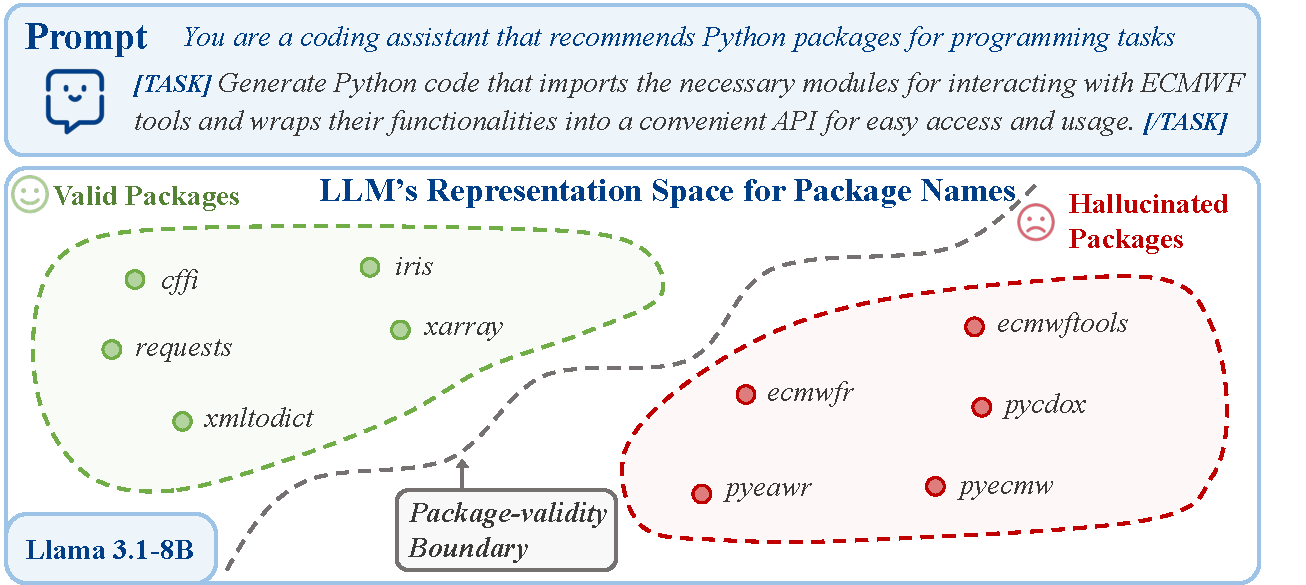
\includegraphics[width=\linewidth]{figure/motivating_example.pdf}
% \captionsetup{skip=2pt}
  \caption{Motivating example of package hallucination as a package-validity boundary problem.}
    \label{fig:motivation}
    % \label{fig:motivating-example}
\vspace{-0.1cm}
\end{figure}

Figure~\ref{fig:motivation} shows a representative package hallucination example from Llama-3.1-8B. 
Given a prompt asking for Python packages to interact with ECMWF tools and wrap their functionalities into a convenient API, the model generates both valid packages, such as \texttt{cffi} and \texttt{iris}, and non-existent package names, such as \texttt{ecmwfr} and \texttt{pyeawr}. 
Because these hallucinated names appear plausible under the task context, developers or automated coding agents may mistakenly treat them as valid dependencies, leading to installation failures or software supply chain risks if attackers register malicious packages under the same names.

This example shows that package hallucination is not simply caused by a lack of package knowledge. 
The model can identify some valid dependencies, but it still fails to distinguish them from plausible non-existent alternatives. 
We view package hallucination as a package-validity boundary error, where the model's distinction between valid and hallucinated packages is unreliable under a given task context. 
Consequently, mitigation should refine this boundary rather than rewrite a specific package recommendation into a fixed target.

% In real-world software development, developers frequently rely on LLMs to recommend software packages for programming tasks or to generate code that depends on external libraries. In such scenarios, the model needs to understand the task requirements and determine which package names are valid and potentially useful for the task. This decision is challenging because non-existent package names may appear plausible under the given task context.


% Figure~\ref{fig:motivation} illustrates a representative example from Llama-3.1-8B. Given a prompt asking for Python packages to interact with ECMWF tools and wrap their functionalities into a convenient API, the model generates several valid packages, such as \texttt{cffi} and \texttt{iris}, which are available in PyPI and potentially relevant to the task. However, the same response also contains non-existent package names, such as \texttt{ecmwf} and \texttt{pyeawr}. Because these hallucinated packages appear plausible in the given context, developers or automated coding agents may mistakenly treat them as valid packages. Such recommendations can lead to installation failures or even software supply chain risks if attackers register malicious packages under the hallucinated names.


% This example suggests that package hallucination is not simply caused by a lack of package knowledge. Although the model can identify some valid and useful dependencies, it may still fail to distinguish valid packages from non-existent but plausible alternatives. We therefore view package hallucination as a package-validity boundary error, where the model's distinction between valid and hallucinated packages becomes unreliable under a given task context. Consequently, mitigating package hallucination should focus on refining the model's package-validity boundary rather than rewriting a specific package recommendation into a fixed target.


\subsection{Task Definition}
We formulate the task of package hallucination mitigation through model editing in the context of package recommendation. 
Let $M_{\theta}$ denote a pretrained LLM with parameters $\theta$. Given a package recommendation prompt $x$, the model generates an answer $a \sim M_{\theta}(x)$, from which we extract a set of package names $P(a)$. Based on a package-validity checking procedure, the extracted packages are partitioned into valid packages $G(a)$ and hallucinated packages $H(a)$:
\begin{equation}
    P(a) = G(a) \cup H(a), \quad G(a) \cap H(a) = \emptyset .
\end{equation}



A package hallucination occurs when $H(a)\neq\emptyset$, meaning that the answer contains at least one hallucinated package. 
For the $i$-th case for model editing, let $a_i \sim M_{\theta}(x_i)$ be the original model response. 
We define the edit case as
\begin{equation}
    e_i = (x_i, G_i, H_i),
    \quad
    G_i = G(a_i),
    \quad
    H_i = H(a_i).
\end{equation}
where $G_i$ denotes valid package recommendations to be preserved or encouraged, and $H_i$ denotes hallucinated package recommendations to suppress.

The goal is to learn an edit $\Delta$ such that the edited model $M_{\theta+\Delta}$ reduces the likelihood of generating hallucinated packages while preserving valid package recommendations:
\begin{equation}
    M_{\theta+\Delta}(x_i) \rightarrow G_i,\quad
    M_{\theta+\Delta}(x_i) \not\rightarrow H_i.
\end{equation}

% This task differs from conventional factual model editing. Instead of rewriting a single subject-object association, package hallucination mitigation requires boundary editing: correcting a task-conditioned boundary between valid and non-existent package names.
